\documentclass[12pt,a4paper]{report}
\usepackage[top=23.4mm, bottom=32mm, left=37mm, right=23.4mm]{geometry}
\usepackage{setspace}
\usepackage{times}
\usepackage{fancyhdr}
\usepackage{graphicx}
\usepackage{hyperref}
\usepackage{tocloft}
\usepackage{indentfirst}
\usepackage{float}
\usepackage{enumitem}
\usepackage{tikz}
\usetikzlibrary{positioning,arrows.meta}
\hypersetup{hidelinks}

% Set Times New Roman font
\renewcommand{\familydefault}{\rmdefault}

% Main text: Times Roman 12pt, justified, 1.5 line spacing
\setstretch{1.5}
\raggedbottom

% Header and Footer setup
\pagestyle{fancy}
\fancyhf{}
\chead{\fontsize{10}{12}\selectfont RasoAI: Ingredient-Based Recipe Recommendation}
\cfoot{\fontsize{10}{12}\selectfont PCU, Department of CSE, 2026-27}
\rfoot{\thepage}
\lfoot{}
\renewcommand{\headrulewidth}{0pt}
\renewcommand{\footrulewidth}{0pt}

% Chapter formatting - 14pt bold CAPITAL with chapter number in front
\usepackage{titlesec}
\titleformat{\chapter}[hang]
  {\fontsize{14}{16}\bfseries}
  {\thechapter.\quad}{0pt}
  {\MakeUppercase}
  
\titlespacing{\chapter}{0pt}{0pt}{24pt}

% Section formatting - 12pt bold left-aligned capitalized
\titleformat{\section}[hang]
  {\fontsize{12}{14}\bfseries}
  {\thesection\quad}{0pt}
  {}
  
\titlespacing{\section}{0pt}{12pt}{6pt}

% Subsection formatting - title case left-aligned
\titleformat{\subsection}[hang]
  {\fontsize{12}{14}}
  {\thesubsection\quad}{0pt}
  {}
  
\titlespacing{\subsection}{0pt}{6pt}{0pt}

% Custom settings
\setcounter{secnumdepth}{3}
\setcounter{tocdepth}{3}

% Figure captions: 12pt for title
\usepackage{caption}
\captionsetup[figure]{font=small, labelsep=period}

% Paragraph indentation (5 spaces = ~0.5 inches)
\setlength{\parindent}{0.5in}
\setlength{\parskip}{6pt}
\setlist{topsep=4pt,itemsep=3pt,parsep=0pt,partopsep=0pt}

% Remove chapter number from page count
\usepackage{etoolbox}
\patchcmd{\chapter}{\thispagestyle{plain}}{\thispagestyle{fancy}}{}{}

\begin{document}

% ==================== FRONT MATTER ====================
% Use Roman numerals for front matter pages

\pagenumbering{roman}
\setcounter{page}{1}

\begin{center}
{\Large TECHNICAL SEMINAR REPORT}\\[0.12in]
{\LARGE\bfseries RasoAI: INGREDIENT-BASED INDIAN RECIPE RECOMMENDATION SYSTEM}\\[0.12in]
{\Large Group ID: \textbf{F12}} \\
\vspace{0.12in}
{FOR THE DEGREE OF}\\[0.12in]
{\bf \large BACHELOR OF TECHNOLOGY}\\[0.12in]
{\bf IN}\\[0.12in]
{\bf COMPUTER SCIENCE AND ENGINEERING}\\[0.12in]
{\it SUBMITTED BY}\\[0.08in]
\begin{tabular}{c}
Shardul Kamde (PRN No.: SOE24201010462)\\
Samvat Jain (PRN No.: SOE24201010443)\\
Abhishek Ghatti (PRN No.: SOE24201010154)\\
Aryan Singh (PRN No.: SOE24201010045)\\
\end{tabular}\par
\vspace{0.1in}
{\it UNDER THE GUIDANCE OF}\\[0.08in]
{\bf \large Dr. Amruta Hingmire}\\[0.12in]

\includegraphics[width=2.2in]{PCU-logo.png}\\[0.12in]
{\bf \small SCHOOL OF ENGINEERING AND TECHNOLOGY}\\
{\bf \small DEPARTMENT OF COMPUTER SCIENCE ENGINEERING}\\
{\large PIMPRI CHINCHWAD UNIVERSITY}\\
{\small 49/50, Plot No. 44, Mohitewadi Rd, Mohitewadi,}\\
{\small Maharashtra 412106}\\[0.08in]
{\bf \footnotesize YEAR 2026-27}\\
\end{center}
\thispagestyle{empty}
% ==================== CERTIFICATE ====================
\clearpage
\thispagestyle{fancy}

\begin{center}


\includegraphics[width=1.65in]{PCU-logo.png}

\vspace{0.45\baselineskip}

{\fontsize{21}{24}\bfseries CERTIFICATE}

\vspace{0.8\baselineskip}

{\fontsize{12}{14}\selectfont
This is to certify that the seminar report entitled
}

\vspace{0.5\baselineskip}

{\fontsize{12}{14}\bfseries
RasoAI: Ingredient-Based Indian Recipe Recommendation System
}

\vspace{1\baselineskip}

{\fontsize{12}{14}\selectfont
Submitted by
}

\vspace{0.5\baselineskip}

{\fontsize{12}{14}\bfseries
Shardul Kamde (PRN No.: SOE24201010462), Samvat Jain (PRN No.: SOE24201010443), Abhishek Ghatti (PRN No.: SOE24201010154),\\
and Aryan Singh (PRN No.: SOE24201010045)
}

\vspace{0.5\baselineskip}

{\fontsize{12}{14}\selectfont
are bona fide students of this institute and the work has been carried out by them under the
supervision of Dr. Amruta Hingmire and is approved for the partial fulfillment of the requirement
of PIMPRI CHINCHWAD UNIVERSITY, for the award of Third Year of Bachelor of
Technology (CSE) A.Y.-2026-27.
}

\vspace{2.1\baselineskip}

% ----------- SIGNATURES IN ONE ROW -----------

\begin{tabular}{ccc}

\begin{minipage}[t]{0.29\textwidth}
\centering
{\fontsize{12}{14}\selectfont Dr. Amruta Hingmire}\\
{\fontsize{12}{14}\selectfont Guide}\\
{\fontsize{12}{14}\selectfont Department of CSE}
\end{minipage}

&

\begin{minipage}[t]{0.29\textwidth}
\centering
{\fontsize{12}{14}\selectfont Ms. Rajashree Landage}\\
{\fontsize{12}{14}\selectfont Technical Seminar Coordinator}\\
{\fontsize{12}{14}\selectfont Department of CSE}
\end{minipage}

&

\begin{minipage}[t]{0.29\textwidth}
\centering
{\fontsize{12}{14}\selectfont Dr. Pallavi Ahire}\\
{\fontsize{12}{14}\selectfont Head of Department}\\
{\fontsize{12}{14}\selectfont Department of CSE}
\end{minipage}

\end{tabular}

\end{center}

\vspace{1\baselineskip}

\noindent
{\fontsize{12}{14}\selectfont
Place: \underline{\hspace{2in}} \hfill Date: \underline{\hspace{1.5in}}
}

\clearpage
% ==================== ACKNOWLEDGEMENT ====================
\begin{center}
{\fontsize{14}{16}\bfseries ACKNOWLEDGEMENT}
\end{center}

\vspace{1\baselineskip}

{\fontsize{12}{14}\selectfont 

\indent We express our sincere thanks to our project guide for valuable suggestions, encouragement, and support throughout the development of RasoAI. The guidance helped us shape the project scope, refine the recipe-matching workflow, and complete this seminar report.

\indent We also thank our Technical Seminar Coordinator, Ms. Rajashree Landage, Academic Coordinator Dr. Sandip Sonawane, Head of the Department Dr. Pallavi Ahire, and Vice Chancellor Dr. Santosh S. Sonavane for their guidance and for providing the academic environment in which this work could be completed.

\indent Finally, we thank our department and our families for their encouragement and support.

}

\vspace{1\baselineskip}
\begin{flushleft}
{\fontsize{12}{14}\bfseries Shardul Kamde}\\
{\fontsize{12}{14}\bfseries Samvat Jain}\\
{\fontsize{12}{14}\bfseries Abhishek Ghatti}\\
{\fontsize{12}{14}\bfseries Aryan Singh}\\
{\fontsize{12}{14}\selectfont Students, Department of CSE}
\end{flushleft}

\clearpage

% ==================== ABSTRACT ====================
\begin{center}
{\fontsize{14}{16}\bfseries ABSTRACT}
\end{center}

\vspace{1\baselineskip}

{\fontsize{12}{14}\selectfont 
\indent RasoAI is a local recipe-finding application that recommends an Indian recipe from ingredients supplied by a user. The project addresses the practical problem of finding a usable recipe when a person has ingredients available but does not know which dish to prepare. Its recipe collection is stored in an Excel workbook containing recipe names, ingredients, instructions, cuisine, course, diet, preparation and cooking times, servings, and source URLs.

\indent The system combines a Streamlit web interface with a FastAPI backend. The backend loads the workbook with pandas and OpenPyXL, normalizes ingredient text, and uses RapidFuzz string similarity to accommodate small spelling variations. A recipe is considered only when at least half of the entered ingredients match; eligible recipes are ranked by ingredient coverage and a keyword-overlap score. The application returns recipe details and dataset instructions, which the interface presents as numbered, gradually revealed steps. The implementation is a deterministic retrieval system: it does not generate recipes with a large language model. Unit tests cover exact ingredient matching, spelling variation, ranking, and insufficient ingredient coverage.
}

\clearpage

% ==================== TABLE OF CONTENTS ====================
\begingroup
\setstretch{1.0}
\small
\tableofcontents
\endgroup

\clearpage

% ==================== MAIN MATTER ====================
% Switch to Arabic numerals starting from Introduction
\pagenumbering{arabic}
\setcounter{page}{1}

\chapter{Introduction}

\section{Overview}
\label{sec:intro_overview}

RasoAI is a local, ingredient-based recipe recommendation system. A user selects ingredients from searchable choices derived from the recipe workbook or enters custom ingredients. The Streamlit frontend sends the selection to a FastAPI service, which searches the recipes loaded from the Excel dataset and returns the best eligible match.

The application has three main responsibilities: presenting and validating user input, retrieving a suitable recipe, and displaying the recipe's source data. The interface shows recipe metadata, the dataset ingredient list, the original recipe URL, and the instructions. Instructions are separated into readable numbered steps; the recipe content itself is sourced from the workbook rather than generated by an LLM.

\section{Motivation}
\label{sec:intro_motivation}

Recipe discovery is often organized around a dish name or a single search phrase. That approach is less helpful when the user starts with ingredients already on hand. RasoAI reverses the search process: it accepts the available ingredients first and ranks recipes according to how well they match that list.

This project was selected to apply data processing, text normalization, approximate string matching, API design, and user-interface development to a familiar real-world task. Its local dataset and local services also make the demonstrated workflow usable without calling a hosted generative-AI service.

\section{Problem Statement and Objectives}
\label{sec:intro_problem}

\textbf{Problem statement:} Given a list of ingredients supplied by a user, identify and present a relevant recipe from a structured Indian-food dataset, while tolerating limited spelling variation and avoiding unsupported recipe generation.

\textbf{Objectives:}
\begin{enumerate}
  \item Load and validate recipe records from the Excel workbook.
  \item Provide searchable dataset ingredients and custom ingredient entry.
  \item Match and rank recipes using approximate keyword comparison and minimum coverage.
  \item Return recipe details through the API and present them with numbered instructions.
  \item Validate matching behavior with automated unit tests.
\end{enumerate}

\section{Scope}
\label{sec:intro_scope}

The current system is a single-user local application backed by a static Excel workbook. It searches the records in that workbook and returns one best match. Users can select from dataset-derived suggestions or provide comma-separated custom ingredients. The API exposes a recipe-search endpoint and an endpoint for ingredient suggestions.

The project does not include user accounts, personalization, ratings, pantry persistence, nutritional analysis, a relational database, live web scraping, or automatic recipe generation. The dataset determines the available recipes and source URLs; updating or expanding the dataset requires updating the workbook. The matching score is a lexical ranking aid, not a measure of recipe quality, dietary suitability, or nutritional safety.

\section{Methodologies of Problem Solving}
\label{sec:intro_methodology}

\begin{enumerate}
  \item \textbf{Data preparation:} inspect required workbook fields, load recipes, normalize ingredients, and derive keywords.
  \item \textbf{Matching:} compare query and recipe keywords with RapidFuzz; enforce 50\% coverage and rank by coverage and overlap.
  \item \textbf{Integration:} provide ingredient suggestions and recipe search through FastAPI, with selection and results in Streamlit.
  \item \textbf{Validation:} test exact and approximate matches, ranking, and insufficient ingredient coverage.
\end{enumerate}

\chapter{Literature Survey}
\label{chap:literature}

Recommender systems select or rank items according to signals that connect a user or query to candidate items. The general design literature distinguishes content-based approaches, which compare item attributes, from collaborative approaches, which use interactions among users and items \cite{recsys}. RasoAI is content-based: recipe ingredient keywords are compared with the ingredients in the query. It does not collect user ratings or interaction history and therefore does not implement collaborative filtering.

Information retrieval systems commonly normalize query and document terms before comparing them. This reduces irrelevant surface variation and enables a term-based comparison \cite{ir}. RasoAI applies a lightweight version of this idea: punctuation and quantities are removed, common measurement and preparation words are excluded, and the remaining ingredient keywords are compared. This design is appropriate for a small local recipe-search workflow, but normalization can also lose context; multiword ingredient phrases are therefore treated as the set of meaningful words extracted from that phrase.

Exact string comparison is brittle when a user makes a small spelling error. Approximate string matching addresses this issue by measuring character-level similarity; RapidFuzz provides the ratio-based comparison used by this implementation \cite{rapidfuzz}. RasoAI accepts a keyword match at a ratio of at least 90 and requires at least half of the entered ingredient items to match a candidate recipe. The threshold is an implementation choice and should be evaluated on additional labelled queries before being treated as an optimal value.

FastAPI provides the HTTP interface between the user-facing application and the recipe-search logic \cite{fastapi}. Streamlit supplies the interactive ingredient-selection interface and result display \cite{streamlit}. Pandas and OpenPyXL provide workbook ingestion and spreadsheet support \cite{pandas,openpyxl}. In contrast to a generative chatbot, this system returns records from a fixed dataset; this makes the provenance of the recipe instructions explicit and avoids presenting newly generated directions as source material.

\chapter{Hardware/Software Requirements Specification}
\label{chap:requirements}

\section{System Requirements}
\label{sec:sys_req}

\subsection{Database Requirements}
\label{subsec:db_req}

RasoAI does not use a database server. Its data store is the supplied Excel workbook, \texttt{backend/data/IndianFoodDatasetXLS.xlsx}. At startup, pandas reads the workbook and the backend constructs an in-memory list of recipe records. The required columns include recipe identifier, name, ingredients, instructions, cuisine, course, diet, preparation time, cooking time, total time, servings, and URL. Keyword sets are derived from the ingredient text. The application is read-only: it does not write user selections or recipe changes to the workbook.

\subsection{Software Requirements (Platform Choice)}
\label{subsec:soft_req}

\begin{itemize}
  \item \textbf{Language and runtime:} Python 3.10 or later.
  \item \textbf{Backend:} FastAPI, Pydantic, and Uvicorn.
  \item \textbf{Frontend:} Streamlit and Requests.
  \item \textbf{Data access:} pandas and OpenPyXL for reading the Excel workbook.
  \item \textbf{Approximate matching:} RapidFuzz.
  \item \textbf{Testing:} Python \texttt{unittest}.
  \item \textbf{Version control:} Git and GitHub.
\end{itemize}

The backend and frontend dependencies are listed separately in their respective \texttt{requirements.txt} files. The backend is started from the \texttt{backend} directory so its relative dataset path resolves correctly; the Streamlit application is started from the \texttt{frontend} directory.

\subsection{Hardware Requirements}
\label{subsec:hard_req}

The application is intended for a general-purpose computer capable of running Python and a modern web browser. It requires local storage for the Excel workbook, source files, Python packages, and optional background video. No GPU or specialized hardware is required. The exact memory and storage requirements depend on the Python environment and local dataset; a fixed hardware benchmark was not part of this project.

\section{Analysis Models: SDLC Model to be Applied}
\label{sec:sdlc}

The project was developed using an iterative, incremental workflow. The dataset loader and matching logic were implemented first, followed by API endpoints, the interactive interface, and result presentation. Each increment could be run locally and checked before further interface or documentation work was added. Unit tests were used to validate important matching rules. This workflow suited the project because the user experience and ranking behavior could be refined as the data and end-to-end application were exercised.

\chapter{System Design}
\label{chap:design}

\section{System Architecture}
\label{sec:architecture}

\begin{figure}[H]
\centering
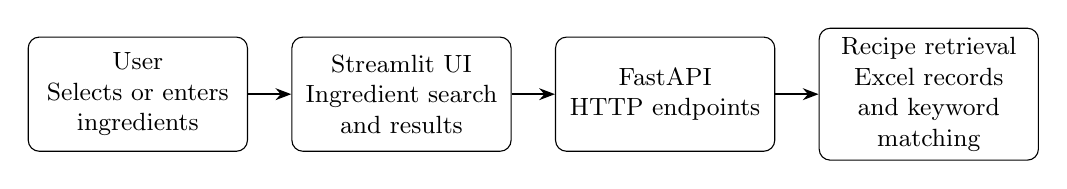
\begin{tikzpicture}[
  node distance=0.55cm,
  component/.style={
    draw,
    rounded corners,
    align=center,
    text width=2.55cm,
    minimum height=1.45cm,
    font=\small
  },
  flow/.style={-{Stealth[length=2mm]}, thick}
]
  \node[component] (user) {User\\Selects or enters ingredients};
  \node[component, right=of user] (ui) {Streamlit UI\\Ingredient search and results};
  \node[component, right=of ui] (api) {FastAPI\\HTTP endpoints};
  \node[component, right=of api] (engine) {Recipe retrieval\\Excel records and keyword matching};
  \draw[flow] (user) -- (ui);
  \draw[flow] (ui) -- (api);
  \draw[flow] (api) -- (engine);
\end{tikzpicture}
\caption{RasoAI high-level system architecture}
\label{fig:architecture}
\end{figure}

The Excel workbook is loaded when the backend starts. The Streamlit frontend requests dataset-derived ingredient choices from \texttt{GET /ingredients}. On submission, it sends the chosen ingredients as JSON to \texttt{POST /chat}. FastAPI passes the query to the recipe retriever, which compares the query with the in-memory recipe keywords and returns either a best match or a no-match response. The interface displays the recipe metadata, source link, ingredients, and instructions.

This separation keeps the presentation layer independent of the matching implementation. The API can also be inspected through the automatically generated FastAPI documentation at \texttt{/docs}.

\chapter{Implementation}
\label{chap:implementation}

\section{Overview of Technical Seminar--II Modules}
\label{sec:modules}

\begin{itemize}
  \item \textbf{Dataset loader (\texttt{dataset\_loader.py}):} reads the Excel workbook, verifies required columns, and constructs recipe records with normalized ingredient keywords.
  \item \textbf{Text utilities (\texttt{utils.py}):} lowercases ingredient text, removes quantities and punctuation, and filters measurement or preparation terms.
  \item \textbf{Recipe retriever (\texttt{recipe\_retriever.py}):} compares query keywords with each recipe, enforces minimum ingredient coverage, scores eligible candidates, and returns the top match.
  \item \textbf{FastAPI service (\texttt{main.py}):} loads data at startup and implements \texttt{GET /}, \texttt{GET /ingredients}, and \texttt{POST /chat}.
  \item \textbf{Streamlit interface (\texttt{web\_ui.py}):} provides searchable dataset ingredient buttons, custom text entry, recipe search, result details, source link, and a step-by-step instruction display.
  \item \textbf{Automated tests:} verify exact ingredient matching, fuzzy spelling tolerance, ranking behavior, and the minimum coverage rule.
\end{itemize}

\section{Tools and Technologies Used}
\label{sec:tools}

Python provides the application runtime. FastAPI and Pydantic define and validate the JSON API, while Uvicorn serves the backend. The Streamlit frontend renders the interactive application and uses Requests to call the local API. Pandas reads the tabular Excel data, with OpenPyXL as the spreadsheet engine. RapidFuzz performs approximate comparisons between normalized words. Git and GitHub provide version history and remote source-code hosting.

\section{Algorithm Details}
\label{sec:algorithms}

\subsection{Ingredient Normalization and Candidate Eligibility}
\label{subsec:algo1}

The text utility converts each ingredient string to lowercase, removes parenthetical text, digits, punctuation, and repeated whitespace, then filters stop words and short tokens. For each recipe, the loader stores the resulting keywords. At query time, the retriever checks each submitted ingredient against the recipe keyword set. A submitted ingredient is considered matched when every keyword extracted from that ingredient has a sufficiently similar recipe keyword. RapidFuzz ratio scores are compared with a threshold of 90.

\begin{small}
\begin{verbatim}
for each recipe:
    matched = matching query ingredients
    coverage = 100 * matched / query size
    if coverage >= 50: keep recipe
\end{verbatim}
\end{small}

\subsection{Candidate Scoring and Ranking}
\label{subsec:algo2}

Eligible recipes are ranked first by ingredient coverage. When coverage is equal, the retriever uses a Dice-style keyword-overlap score:
\[
\mathrm{score}(U,R) =
\frac{2\,|M(U,R)|}{|U|+|R|}\times 100,
\]
where \(U\) is the set of query keywords, \(R\) is the set of recipe keywords, and \(M(U,R)\) is the number of query keywords that match a recipe keyword under the fuzzy threshold. The score is a lexical similarity indicator; it is not a probability that the recipe will be suitable or successful.

\begin{small}
\begin{verbatim}
best = none; best_rank = (0, 0)
for each eligible recipe:
    rank = (coverage, keyword_overlap)
    if rank > best_rank: update best
return best, or no_match
\end{verbatim}
\end{small}

\chapter{Results}
\label{chap:results}

\section{Result Analysis and Validations}
\label{sec:result_analysis}

The workbook contains 6,871 recipe rows and the columns used by the application for ingredient matching and result display. The backend returns dataset-derived ingredient suggestions and recipe results through its API. The UI was exercised with selected ingredients and custom ingredient input, and displays the best-match metadata, source URL, dataset ingredients, and numbered instructions.

The automated test suite contains four focused tests. Table~\ref{tab:tests} summarizes their intended checks.

\begin{table}[H]
\centering
\caption{Recipe retrieval validation cases}
\label{tab:tests}
\begin{tabular}{|p{0.34\textwidth}|p{0.51\textwidth}|}
\hline
\textbf{Test case} & \textbf{Expected behavior}\\
\hline
Exact ingredient preference & Select the recipe containing the exact requested ingredient rather than a partial-word candidate.\\
\hline
Query-based scoring & Prefer the recipe that best covers the supplied ingredients, not simply the recipe with more ingredient words.\\
\hline
Minimum coverage & Return no recipe when fewer than half of the submitted ingredients match.\\
\hline
Spelling variation & Match a small spelling variation when its fuzzy similarity passes the configured threshold.\\
\hline
\end{tabular}
\end{table}

All four recipe-retriever unit tests pass in the development environment. The threshold and score are heuristic design choices; a larger labelled test set and user evaluation would be needed to quantify recommendation quality beyond these functional tests.

\section{Representative User Workflow}
\label{sec:screenshots}

\begin{enumerate}
  \item Open the Streamlit application after starting the FastAPI backend.
  \item Search for an ingredient or select one of the popular dataset-derived ingredient buttons.
  \item Add optional comma-separated ingredients that are not in the suggestions.
  \item Select \textbf{Generate recipe}.
  \item Review the best recipe match, its cuisine/course/time metadata, the source link, and the dataset ingredients.
  \item Read the instructions as numbered steps, which are revealed one line at a time.
\end{enumerate}

The architecture diagram in Figure~\ref{fig:architecture} documents the implemented data flow. A separate application screenshot is not included in this source file.

\chapter{Conclusions and Future Scope}
\label{chap:conclusion}

\section{Conclusion}
\label{sec:conclusion}

RasoAI demonstrates a local content-based recipe retrieval workflow built from a spreadsheet dataset. It connects a searchable ingredient-selection interface to a FastAPI service, normalizes ingredient text, tolerates small spelling variations, applies a minimum coverage threshold, and returns a ranked recipe record. Recipe instructions and metadata are sourced from the workbook rather than generated by a language model.

The implementation meets its core functional objectives: the dataset is loaded and validated, ingredient choices can be searched and selected, recipe matching is exposed through an API, and the Streamlit interface presents the result in a readable form. Four unit tests validate important matching behaviors. The score remains a heuristic and the application currently returns one best match without personalization.

\section{Future Scope}
\label{sec:future}

\begin{itemize}
  \item Evaluate ranking quality against a larger, manually labelled query set and tune the coverage and fuzzy thresholds from measured results.
  \item Improve ingredient parsing for synonyms, regional names, plural forms, transliterations, and multiword ingredients.
  \item Return several ranked recipe candidates and allow filters for cuisine, course, diet, and preparation time.
  \item Add automated API and browser-level integration tests.
  \item Add optional user accounts, saved ingredient lists, ratings, and personalized ranking if persistent storage is introduced.
  \item Improve accessibility and provide a user-controlled instruction reveal speed.
  \item Add data-update validation and a clear process for refreshing the recipe workbook.
\end{itemize}



% ==================== APPENDICES ====================
\appendix

\chapter{API and Local Execution}
\label{app:publication}

Run the backend from its \texttt{backend} folder and the frontend from its \texttt{frontend} folder:

\begin{verbatim}
python -m pip install -r requirements.txt
python -m uvicorn main:app --reload

streamlit run web_ui.py
\end{verbatim}

\noindent Ingredient suggestions: \texttt{GET /ingredients}.\\
Recipe search: \texttt{POST /chat}.

A recipe search request has this form:

\begin{verbatim}
{
  "ingredients": ["onion", "tomato"]
}
\end{verbatim}

The API documentation is available while the backend is running:

\begin{center}
\url{http://127.0.0.1:8000/docs}
\end{center}

\section{Project Limitations}
\label{app:limitations}

The system depends on the provided workbook and does not verify that a recipe is safe for a particular allergy or dietary condition. Similarity scores are based on normalized text and should not be interpreted as nutritional or culinary guarantees. The current backend loads its dataset into memory at startup, and changes to the workbook require restarting the backend.

% ==================== REFERENCES ====================
\clearpage
\raggedright
\begin{thebibliography}{99}

\bibitem{recsys} Francesco Ricci, Lior Rokach, and Bracha Shapira, editors, \textit{Recommender Systems Handbook}, 2nd ed., Springer, 2015. doi: \href{https://doi.org/10.1007/978-1-4899-7637-6}{10.1007/978-1-4899-7637-6}.

\bibitem{ir} Christopher D. Manning, Prabhakar Raghavan, and Hinrich Sch\"utze, \textit{Introduction to Information Retrieval}, Cambridge University Press, 2008. \url{https://nlp.stanford.edu/IR-book/}.

\bibitem{fastapi} FastAPI, ``FastAPI Documentation.'' \url{https://fastapi.tiangolo.com/}.

\bibitem{streamlit} Streamlit, ``Streamlit Documentation.'' \url{https://docs.streamlit.io/}.

\bibitem{rapidfuzz} RapidFuzz, ``RapidFuzz Documentation.'' \url{https://rapidfuzz.github.io/RapidFuzz/}.

\bibitem{pandas} pandas development team, ``pandas Documentation.'' \url{https://pandas.pydata.org/docs/}.

\bibitem{openpyxl} openpyxl, ``openpyxl Documentation.'' \url{https://openpyxl.readthedocs.io/}.

\end{thebibliography}

\end{document}